\documentclass[a4paper,12pt]{article}
\usepackage[utf8]{inputenc}

\usepackage[utf8]{inputenc}
\usepackage[T2A]{fontenc}
\usepackage[english,russian]{babel}
\usepackage{amsthm}
\usepackage{amsmath}
\usepackage{amssymb}
\usepackage{tikz}
\usepackage{textcomp}
\usepackage{marvosym}
\usepackage{ esint }
\usepackage{mathtext}
\usepackage{siunitx} % Required for alignment
\usepackage{subfigure}
\usepackage{multirow}
\usepackage{rotating}
\usepackage{afterpage}
\usepackage[arrowdel]{physics}
\usepackage{booktabs}
\setlength{\topmargin}{-0.5in}
\setlength{\textheight}{9.1in}
\setlength{\oddsidemargin}{-0.4in}
\setlength{\evensidemargin}{-0.4in}
\setlength{\textwidth}{7in}
\setlength{\parindent}{0ex}
\setlength{\parskip}{1ex}
\newcommand{\ndiv}{\hspace{-4pt}\not|\hspace{2pt}}
\usepackage{graphicx}
\usepackage{float}
\usepackage{wrapfig}
\usepackage{pgfplots}
\usepackage{caption}
\pgfplotsset{compat=1.16}
\graphicspath{ {./images/} }
\usepackage{graphicx}
\RequirePackage{caption}
\DeclareCaptionLabelSeparator{defffis}{ — }
\captionsetup{justification=centering,labelsep=defffis}
\usepackage{caption} \captionsetup[table]{labelsep=endash,justification=justified,singlelinecheck=false,font=normalsize}
\usepackage{amsfonts,mathtools}

\title{Лабораторная работа № 5.1.3\\Эффект Рамзауэра}
\author{Илья Прамский}
\date{Ноябрь 2024}

\begin{document}
\maketitle
\newpage
\section*{Теоретическая справка}
\[E = \frac{mv^2}{2} = \frac{mv'^2}{2}+U\]

\begin{equation}
n = \frac{\lambda}{\lambda'} = \sqrt{1 - \frac{U}{E}}
\end{equation}

После решения соответствующего уравнения Шрёдингера получается выражение для коэффициента прохождения:

\begin{equation}
D = \frac{16 k_1^2 k_2^2}{16k_1^2 k_2^2 + 4\left(k_1^2-k_2^2\right)^2\sin^2\left(k_2 l\right)}
\end{equation}
где $k_1^2 = \frac{2mE}{\hbar^2}, k_2^2 = \frac{2m(E + U_0)}{\hbar^2}$.

Это периодическое выражение с максимумами при 

\begin{equation}
k_2 l = \pi n = \sqrt{\frac{2m(E + U_0)}{\hbar^2}}l
\end{equation}

Выражения для эффективного размера атома $l$:
\begin{equation}
2l = \frac{h}{\sqrt{2m(E_1 + U_0)}}
\end{equation}

\begin{equation}
2l = \frac{3}{2}\frac{h}{\sqrt{2m(E_2 + U_0)}}
\end{equation}

Где $E_1, E_2$ --- энергии, соответствующие максимуму и минимуму прохождения электронов соответственно. Исключая $U_0$ можно найти 

\begin{equation}
l = \frac{h\sqrt{5}}{\sqrt{32m(E_2 - E_1)}}
\end{equation}

А исключая $l$ можно найти эффективную глубину потенциальной ямы атома:

\begin{equation}
U_0 = \frac{4}{5}E_2 - \frac{9}{5}E_1
\end{equation}

Формула, связывающую зависимость вероятности рассеяния электрона от его энергии:
\begin{equation}
w(V) = -\frac{1}{C} \ln \frac{I_a(V)}{I_0}
\end{equation}

\begin{figure}[H]
\begin{center}
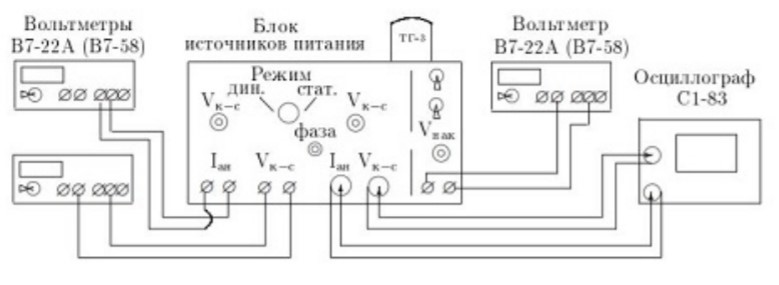
\includegraphics[width = 0.6\textwidth]{scheme.jpg}
\caption{Схема экспериментальной установки}
\end{center}
\end{figure}

\section*{Ход работы}
\subsection*{Динамический режим}
Два графика в динамическом режиме при разном U
\begin{figure}[H]
\begin{minipage}[c]{0.5\textwidth}
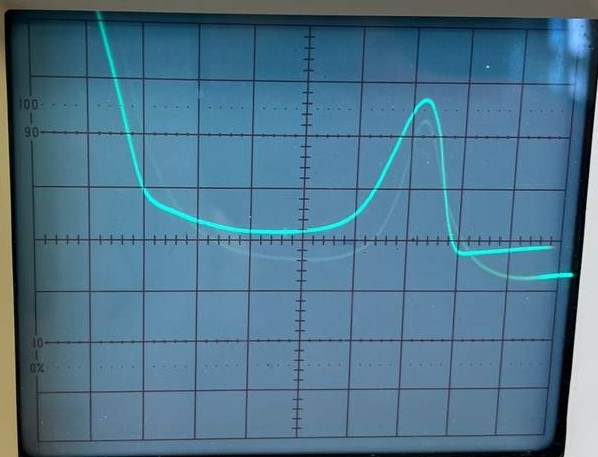
\includegraphics[width = 0.9\textwidth]{graph1.jpg}
\caption{Вольт-амперная характеристика при U=2.63 В}
\end{minipage}
\begin{minipage}[c]{0.5\textwidth}
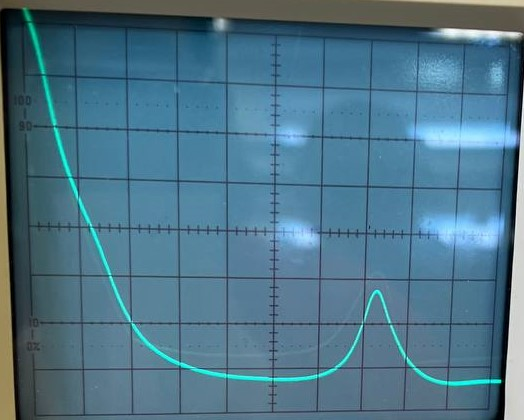
\includegraphics[width = 0.9\textwidth]{graph2.jpg}
\caption{Вольт-амперная характеристика при U=2.5 В}
\end{minipage}
\end{figure}

Получается ($l_1, l_2, l_3$ - по формуле (4),(5), (6) соответственно; $E_n = U_n \cdot e$). 

\begin{table}[H]
\centering
\begin{tabular}{|c|c|c|c|c|c|c|}
\hline
$U_\text{нак}$, В & $U_1$, В & $U_2$, В & $l_1$, \AA & $l_2$, \AA & $l_3$, \AA & $U_0,$ В \\
\hline
2,63 & 1,4 & 6.3 & 3,1 & 3,1 & 3,1 & 2.52 \\
\hline
2,50 & 3.6 & 9.6 & 2.48 & 2.64 & 2.8 & 1.20 \\
\hline
\end{tabular}
\end{table}

\subsection*{Статический режим}
\begin{table}[H]
\centering
\begin{tabular}{|c|c|c|c|}
\hline
\multicolumn{2}{|c|}{U=2.63 В} & \multicolumn{2}{|c|}{U=2.5 В} \\
\hline
U, В & $U_a$, мВ & U, В & $U_a$, мВ \\
\hline
0,30 &	3,00 & 0,3 &	3,00 \\
\hline
0,60 &	30,60 & 0,97	& 103,00 \\
\hline
0,90 &	93,00 & 1,35	& 160,00 \\
\hline
1,00 &	114,00 & 1,49	& 170,65 \\
\hline
1,07 &	126,50 & 1,62	& 175,50 \\
\hline
1,20 &	145,00 & 1,79	& 176,10 \\
\hline
1,30 &	158,40 & 1,89	& 174,30 \\
\hline
1,40 &	172,00 & 2,15	& 164,80 \\
\hline
1,60 &	180,00 & 2,70	& 140,00 \\
\hline
1,70 &	181,00 & 3,27	& 121,50 \\
\hline
1,69 &	181,55 & 3,70	& 110,40 \\
\hline
2,07 &	171,00 & 4,27	& 100,50 \\
\hline
2,42 &	155,90 & 5,00 & 	90,30 \\
\hline
2,65 &	145,60 & 5,40 & 	87,55 \\
\hline
3,37 &	125,00 & 5,96 & 	86,40 \\
\hline
4,38 &	111,00 & 7,20 & 	90,90 \\
\hline
5,13 &	105,50 & 8,23	& 100,84 \\
\hline
4,45 &	112,80 & 9,62	& 131,00 \\
\hline
4,95 &	109,00 & 10,83	& 164,00 \\
\hline
5,45 &	107,00 & 11,57	& 190,00 \\
\hline
6,50 &	114,70 & 11,81	& 215,00 \\
\hline
7,13 &	121,00 & & \\
\hline
8,53 &	145,60 & & \\
\hline
10,00 &	197,50 & & \\
\hline
11,90 &	376,00 & & \\
\hline



\end{tabular}
\end{table}

\begin{figure}[H]
\centering
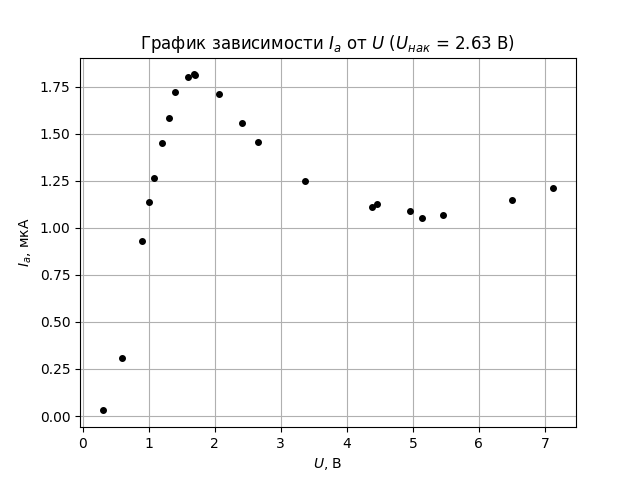
\includegraphics[width = 0.7\textwidth]{graph3.png}
\end{figure}

\begin{figure}[H]
\centering
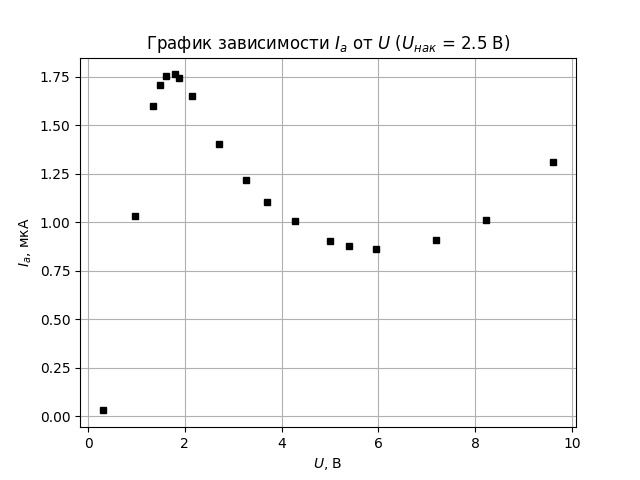
\includegraphics[width = 0.7\textwidth]{graph4.png}
\end{figure}

\begin{table}[H]
\centering
\begin{tabular}{|c|c|c|c|c|c|c|}
\hline
$U_\text{нак}$, В & $U_1$, В & $U_2$, В & $l_1$, \AA & $l_2$, \AA & $l_3$, \AA & $U_0,$ В \\
\hline
2,63 & 1,69 & 5,13 & 3,00 & 3,33 & 3,70 & 1,06 \\
\hline
2,50 & 1,79 & 5,96 & 2,96 & 3,16 & 3,36 & 1,55 \\
\hline
\end{tabular}
\end{table}

График зависимости вероятности рассеяния электронов (с точностью до константы) от энергии.

\begin{figure}[H]
\centering
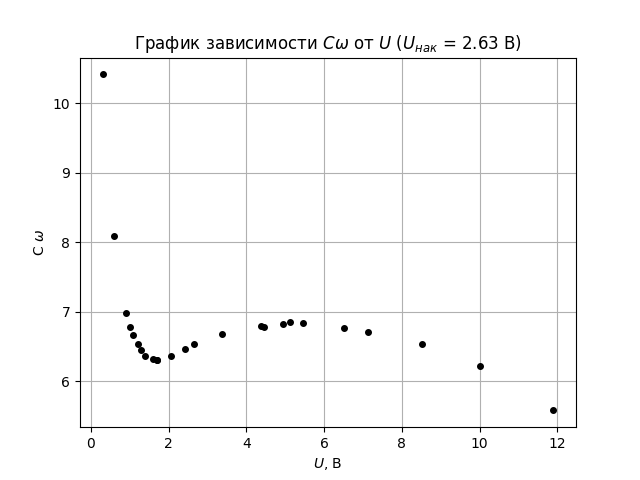
\includegraphics[width = 0.7\textwidth]{graph5.png}
\end{figure}

\begin{figure}[H]
\centering
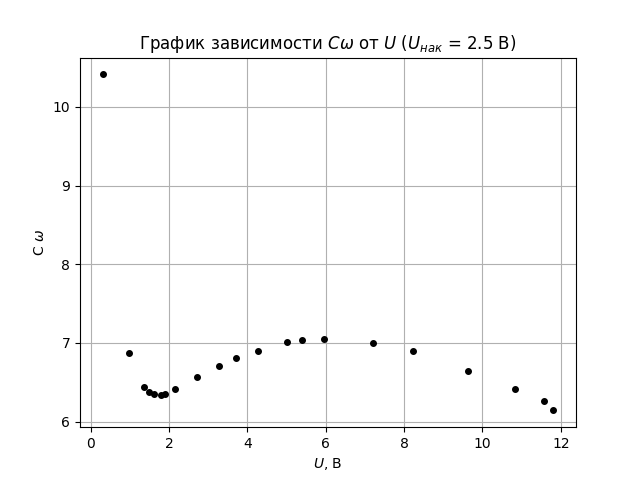
\includegraphics[width = 0.7\textwidth]{graph6.png}
\end{figure}

\section*{Вывод}
В ходе данной работы был исследован эффект Рамзауэра, оценены параметры при разных режимах работы установки. Так, при помощи нескольких формул был оценён размер электронной оболочки атома, причем значения полученных оценок близки к табличному значению удвоенного ковалентного радиуса(2,8 \AA). Также было оценено значение потенциальной ямы, во всех опытах оно совпало по порядку, а в одном из даже оказалось достаточно близко к истинному(U = 2.52). Также была получена зависимость вероятности рассеяния электронов от энергии, которая имеет поведения, похожее на график из методического материала.
\end{document}